\chapter{Review of the state of the art}

\section{Introduction to bottoming recuperative cycles}

A bottoming cycle is a waste-heat recovery thermodynamic cycle that recaptures the unused energy and uses it to produce steam to drive a steam turbine generator to produce additional energy. In Figure~\ref{fig:bottoming} is shown a general configuration for a bottoming cycle. In the passenger case car, the thermal process upstream the cycle is the internal combustion engine itself.

\begin{figure}[ht]
  \centering
  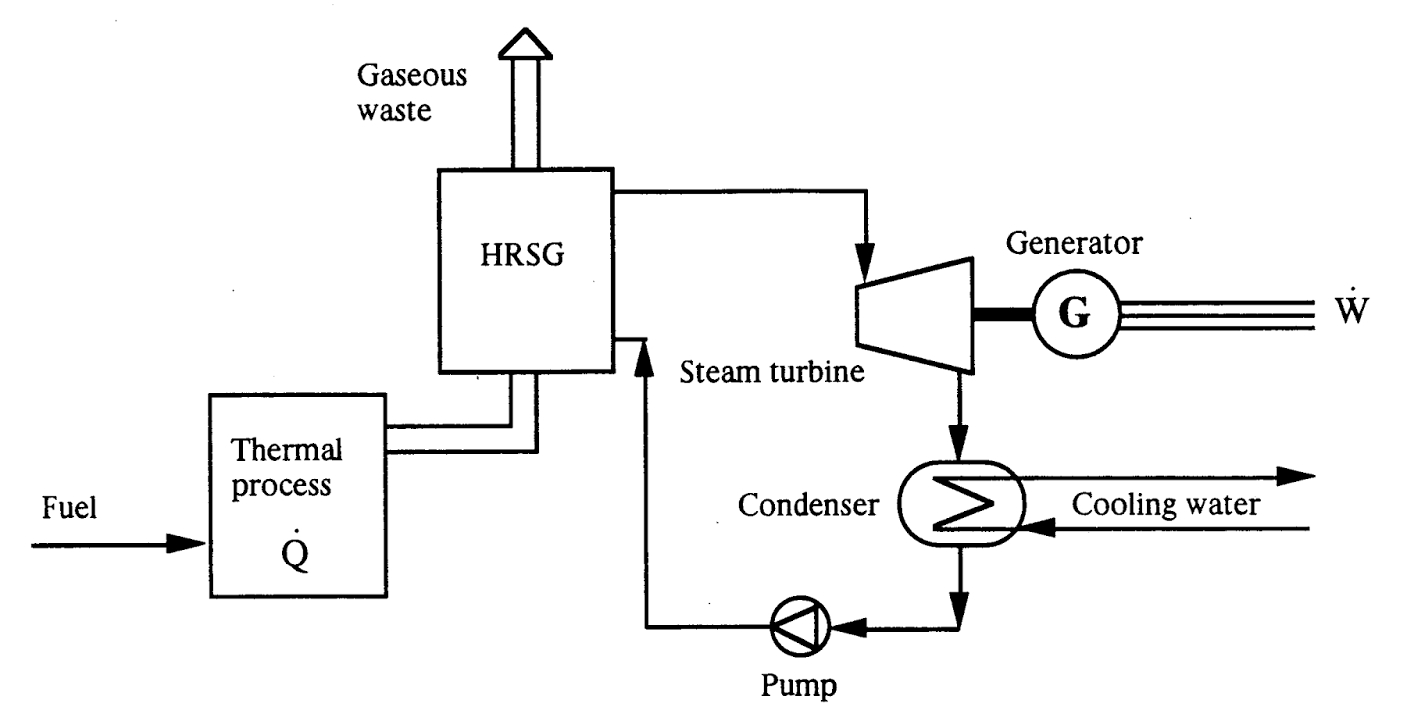
\includegraphics[width=0.7\textwidth]{figures/review/bottoming.jpg}
  \caption{Bottoming cycle \label{fig:bottoming} }
\end{figure}
~

A bottoming cycle is a powerful mean to recover the waste heat produced by an automotive internal combustion engine, and the additional power produced can be employed in different ways. It is possible to produce additional mechanical work, increasing the torque at the shaft, or produce electrical work that can be employed in different ways. Usually the selected recovery strategy is to use the recuperative cycle to produce mechanical power: this implementation is simpler and effective, but fails to achieve the maximum potential with respect to the operative conditions of the additional cycle. In this configuration the angular speed of the turbine is the same as the one of the shaft, but this speed can be different from the one of maximum efficiency of the turbo-machine.

The configuration that converts the additional power in electrical power can solve this issue. Being the system no more coupled with the shaft of the internal combustion engine but with an electric generator, the rotational speed of the turbine can be varied at will in order to achieve the most efficient operative point. The electricity produced can be stored in batteries is they are available (i.e. Hybrid or Plug-in vehicle), or used to power up auxiliaries and reduce the alternator load on the engine.

In the following sections a brief overview of the most common thermodynamic cycles that can be used as a recuperative bottoming cycle will be provided.

\subsection{Steam Rankine cycle}

The steam Rankine cycle is one of the most famous and used thermodynamic cycles for producing power. In this cycle the heat is provided externally to a closed loop, in which water flows as a working fluid. The efficiency of the Rankine cycle can be calculated as:

\begin{equation} \label{eq:eta_rankine}
  \eta_t = \frac{\dot{W}_{thermal}-\dot{W}}{\dot{Q}_{in}} \approx \frac{\dot{W}_{turb}}{\dot{Q}_{in}}
\end{equation}

This type of cycle is commonly used in thermal power generation plants. The efficiency of the Rankine cycle is limited by the high heat of vaporization of the working fluid. Also, unless the pressure and temperature reach super critical levels in the steam boiler, the temperature range the cycle can operate over is quite small: steam turbine entry temperatures are typically around \SI{565}{\celsius} and steam condenser temperatures are around \SI{30}{\celsius}.

\begin{figure}[ht]
  \centering
  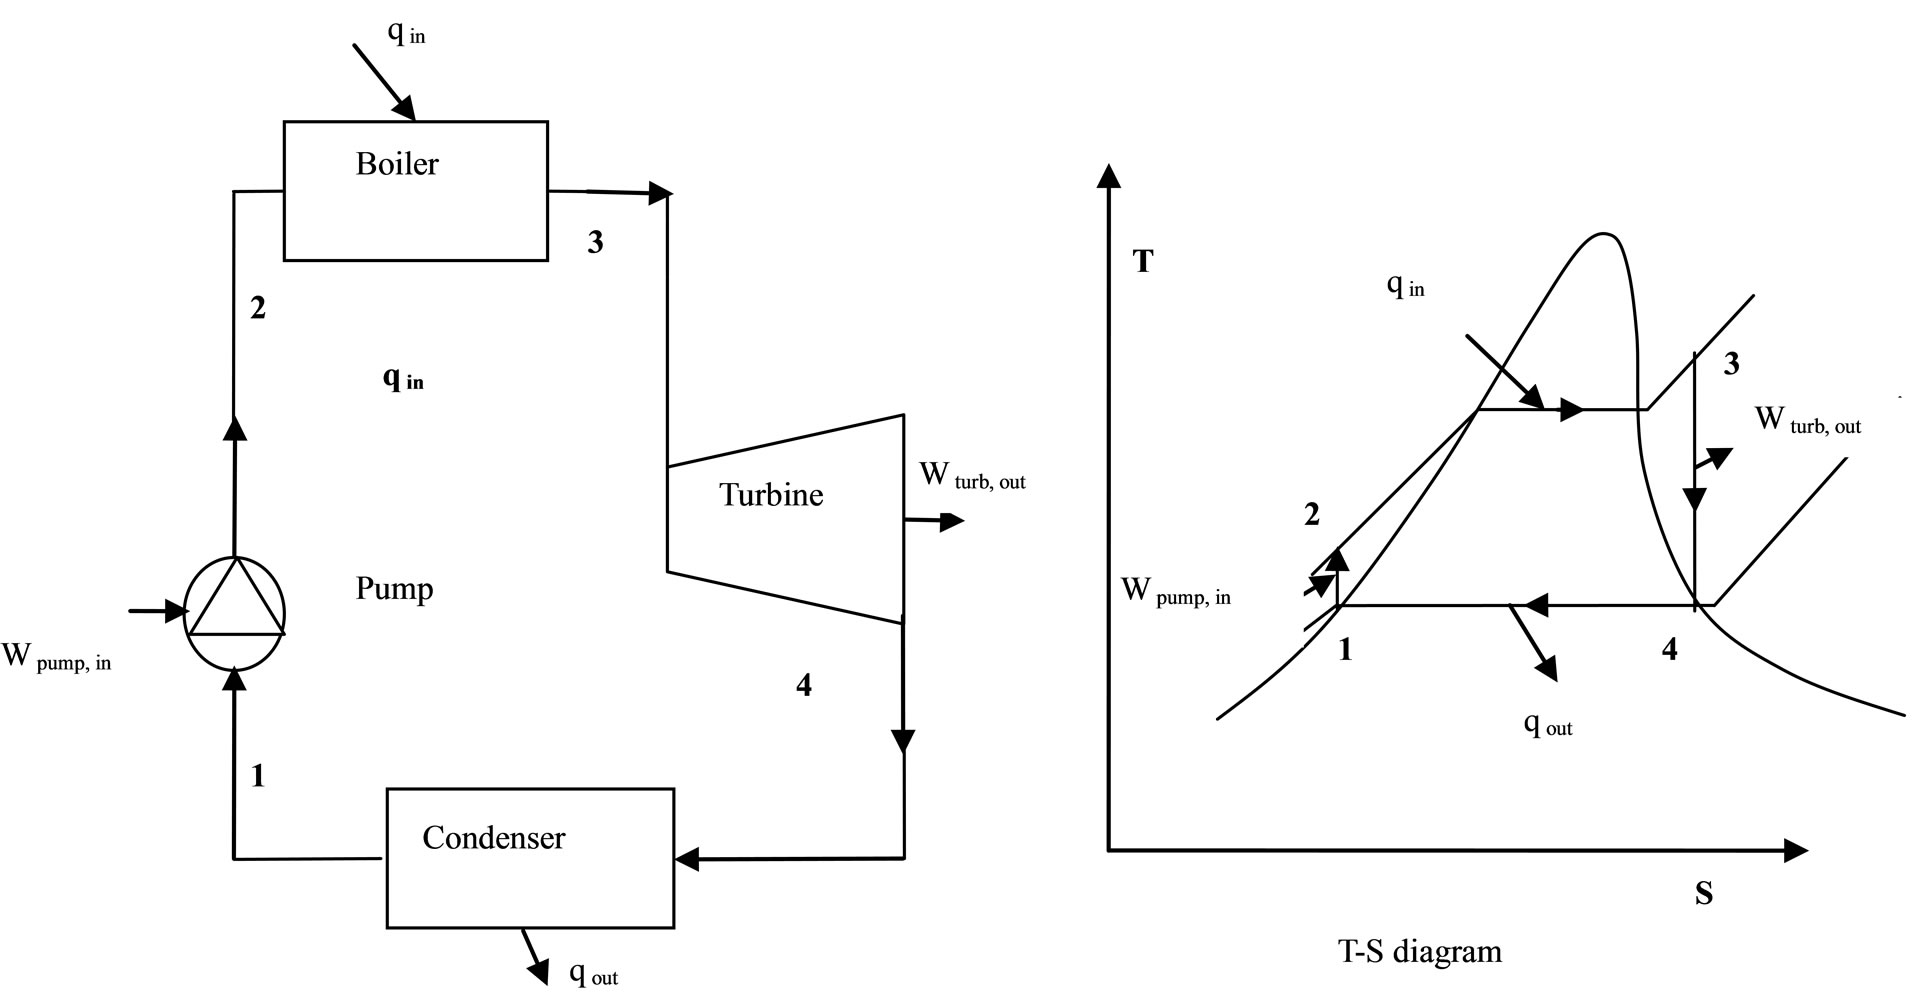
\includegraphics[width=\textwidth]{figures/review/rankine_steam.jpg}
  \caption{Steam Rankine cycle T-s diagram and physical layout\label{fig:rankine_steam} }
\end{figure}

The process is composed by four consecutive processes, as shown in Figure~\ref{fig:rankine_steam}:

\begin{itemize}
\item \textbf{Process 1-2:} the working fluid is pumped from low to high pressure. Since the fluid is in liquid form, the work required for pumping is small.
\item \textbf{Process 2-3:} the liquid at high pressure is heated at almost constant pressure by an external source until it becomes dry saturated vapor.
\item \textbf{Process 3-4:} the dry saturated vapor is expanded through a turbine, hence generating power. The working fluid experience a decrease of pressure and temperature, with possible partial condensation.
\item \textbf{Process 4-1:} the wet vapor enters the condenser and returns to saturated liquid conditions.
\end{itemize}



\subsection{Organic Rankine cycle}

The Organic Rankine Cycle (ORC) is a particular use case of a Rankine thermodynamic cycle. It's named for its use of an organic, high molecular mass fluid with a liquid-vapor phase change, or boiling point, occurring at a lower temperature than the water-steam phase change. The fluid allows Rankine cycle heat recovery from lower temperature sources such as coolant from internal combustion engines. The low-grade waste heat is converted into useful work, that can itself be converted into mechanical or electrical power. In Figure~\ref{fig:orc_diagram}, the T-s diagram and the plant layout for a generic Organic Rankine Cycle are shown. The formulation of the efficiency is the same as the Steam Rankine Cycle, shown in Equation~\ref{eq:eta_rankine}.

\begin{figure}[ht]
  \centering
  \includegraphics[width=0.8\textwidth]{figures/review/orc.jpg}
  \caption{T-s diagram and plant layout for a generic Organic Rankine Cycle\label{fig:orc_diagram} }
\end{figure}

The system itself is made of four components: evaporator, expander, condenser and pump. Usually a recuperator is also used, to increase the efficiency and hence the production of useful power. The waste heat is used in the evaporator to vaporize the working fluid and convert the heat in mechanical work in the expander.

The selection of the working fluid is of key importance in low temperature Rankine Cycles. Because of the low temperature, heat transfer inefficiencies have a major importance. In order to recover low-grade heat, the fluid generally has a lower boiling temperature than water, then refrigerants and hydrocarbons are two commonly used components. Water is a preferable working fluid for high exhaust gas temperatures ranging from \SI{500}{\celsius} to \SI{800}{\celsius}, while refrigerants are better suited fro lower temperatures, as in the gas of the exhaust gases. Water also has the disadvantage that requires superheating to avoid turbine blade erosion, but the high degree of superheating makes it less practical for automotive application due to the variation of exhaust temperature at different load conditions. In figure~\ref{fig:orc_working_fluids} are reported the different T-s diagram related to different Rankine cycle working fluids.

\begin{figure}[ht]
  \centering
  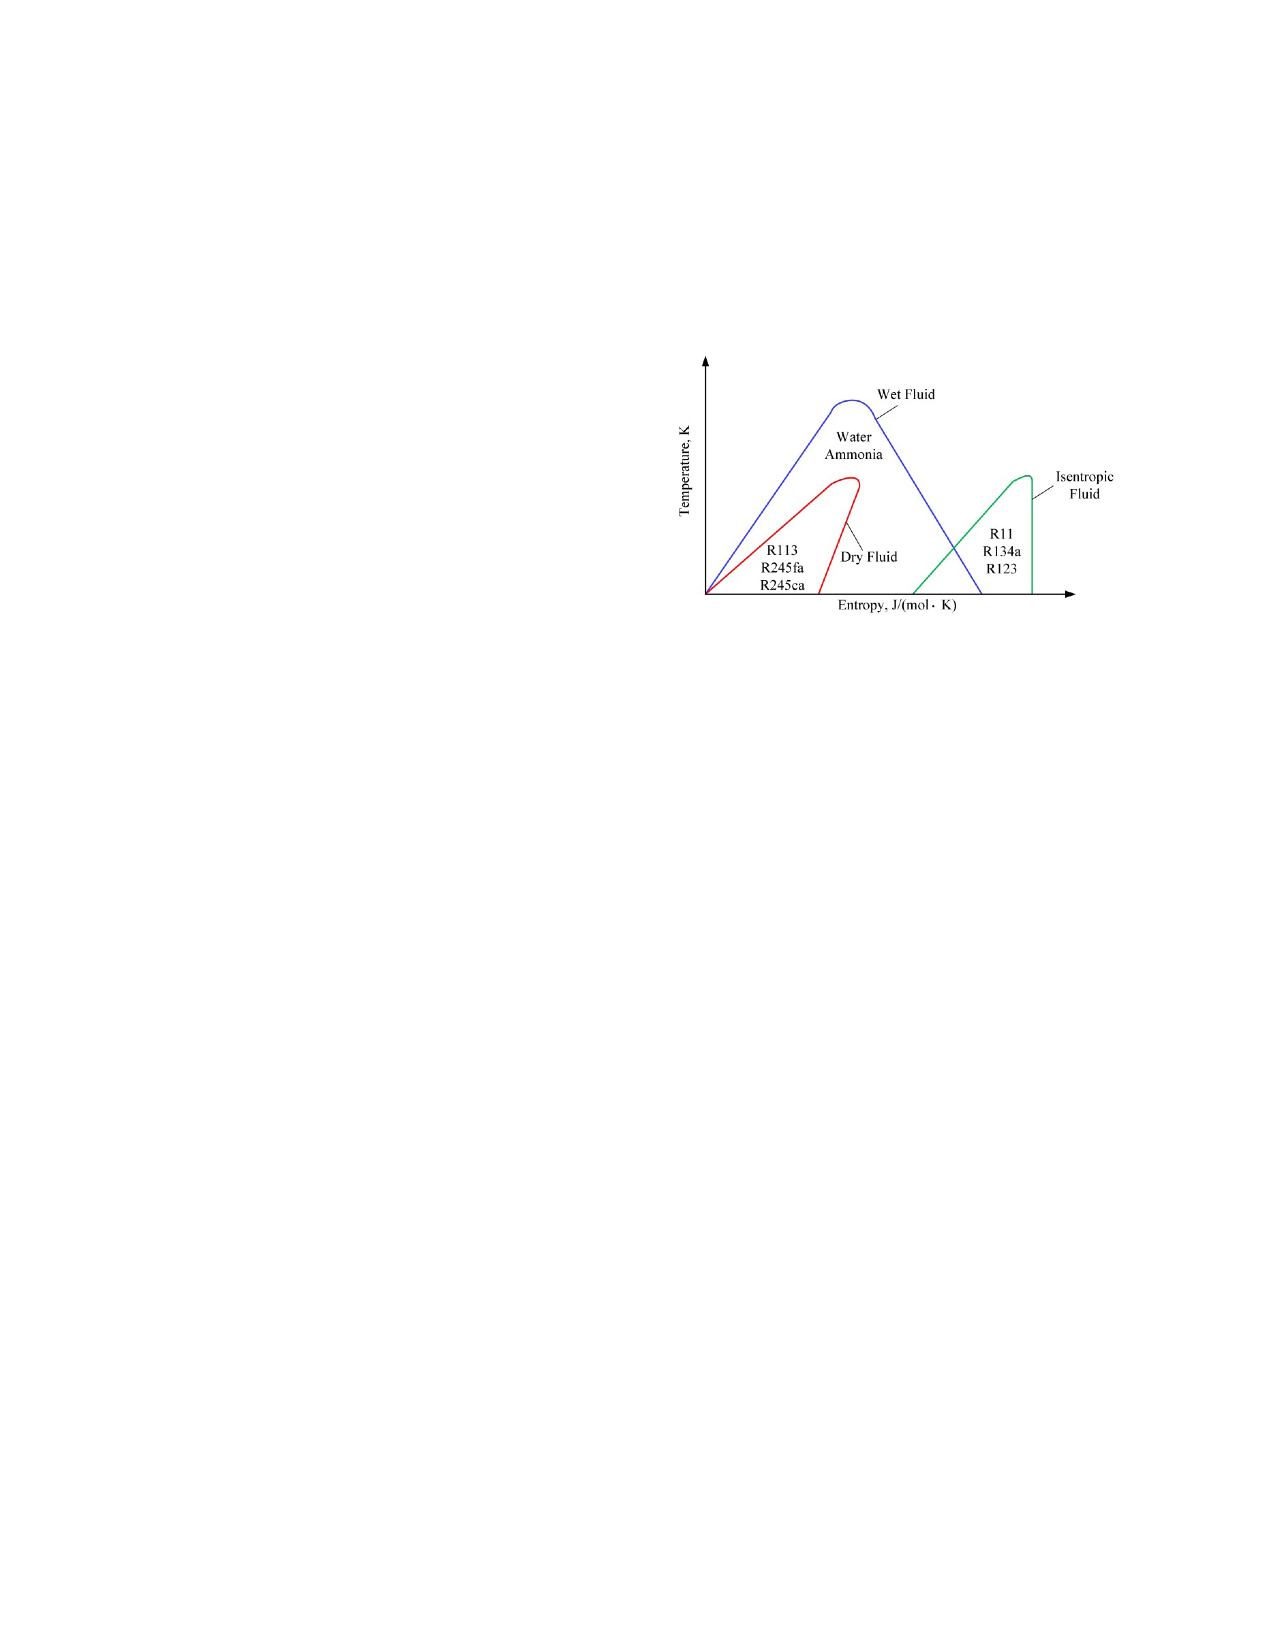
\includegraphics[width=0.7\textwidth]{figures/review/orc_working_fluids.pdf}
  \caption{Comparison of different Rankine Cycle working fluid characteristics\label{fig:orc_working_fluids} }
\end{figure}

In current years, an increasing environmental awareness has provoked the shifting from traditional refrigerants (i.e. R134a, R236fa, R245fa) to new refrigerants, characterized by lower harm potential to passengers in case of leakage or crashes, and a lower flammability level (i.e. R1233zd, R1234yf).

When considering an ORC coupled with an internal combustion engine, different possible configurations must be considered. The most common and simple structure utilizes the exhaust gas as the only heat source to evaporate the working fluid. The second structure adds another heat exchanger (recuperator) before the evaporator, using the steam from the expander to preheat the working fluid. A third structure uses waste heat from engine coolant to preheat the working fluid. The regenerative preheating of structure 2 requires a very complex liquid-gas heat exchanger with high exchange surfaces, while the preheater in structure 3 only requires a simple liquid-liquid heat exchanger. There have been contradicting conclusions about the effect of preheating using engine coolant on the RC system efficiency. Based on Vaja and Gambarotta's work \cite{Vaja2010}, the RC system with a preheater allows a net increase in power output, compared to structure 1, of 10\% to 35\%, depending on which working fluid is chosen. Alberto Boretti \cite{Boretti2012} also showed a 8.2\% fuel economy improvement using engine coolant to preheat the RC cycle, compared to a 6.4\% improvement when only exhaust gas is used to boil the working fluid. Arias et al. \cite{Arias2006} also compared the combined exhaust and engine coolant heat recovery system with the exhaust only structure. It was found that the additional power recovered from the engine coolant system was 20 W out of a total 2140 W, which is around 1\% improvement.

\begin{figure}[ht]
  \centering
  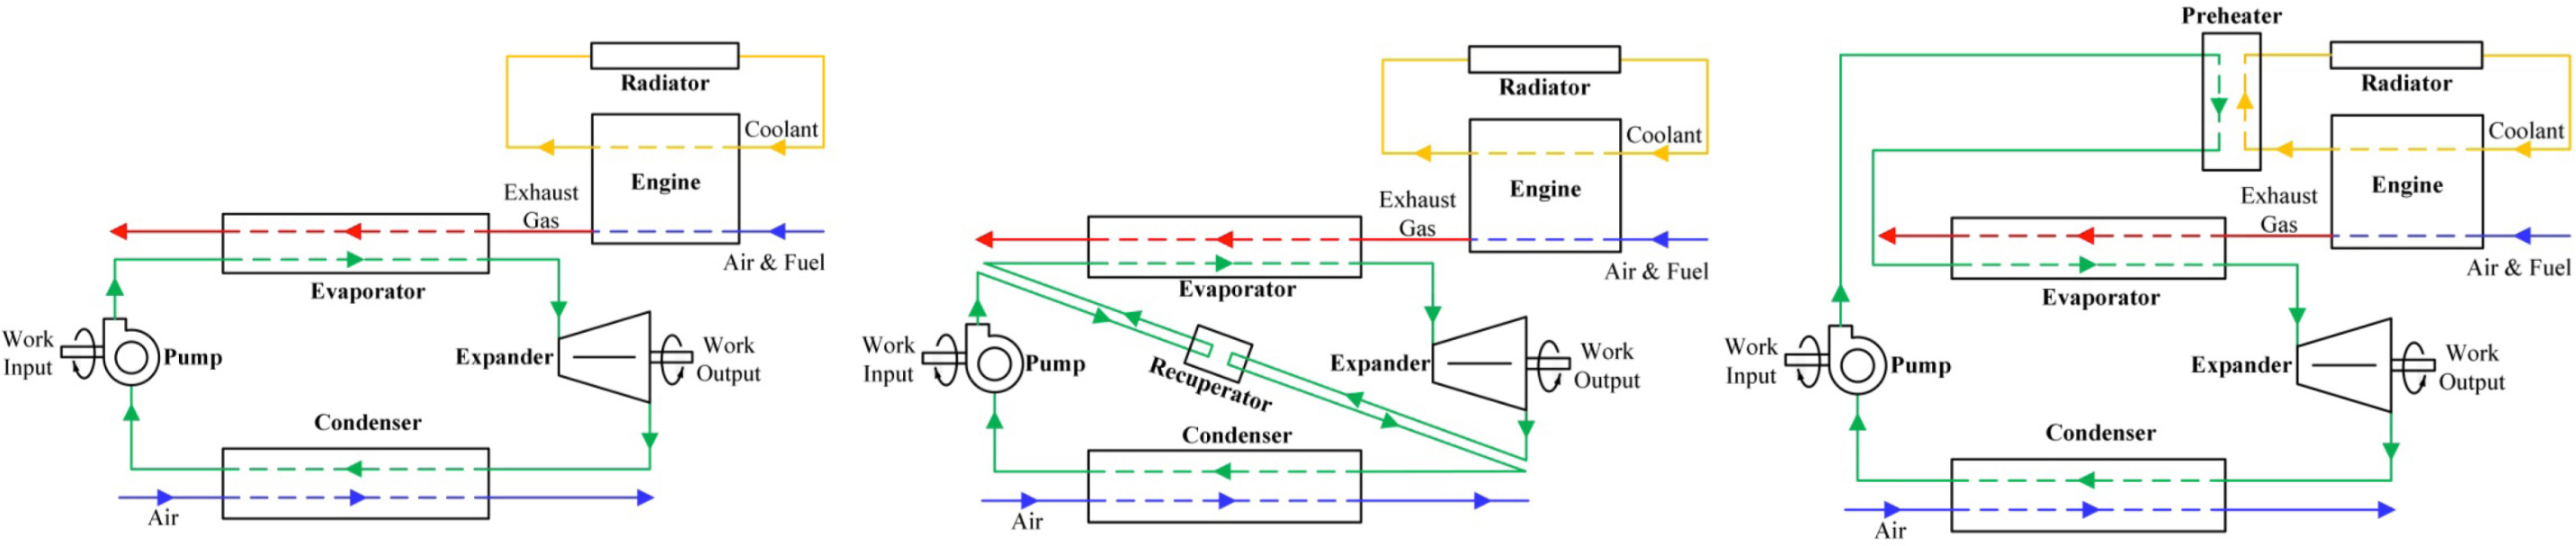
\includegraphics[width=\textwidth]{figures/review/orc_layouts.jpg}
  \caption{Different ORC layouts: structure 1, 2 and 3\label{fig:orc_layouts} }
\end{figure}

When selecting the different configurations, different factors have to be take into consideration as the maximization of the recovered energy is not the only objective to pursue. System complexity, component volume and weight, and the resulted extra cost added to the vehicles and the payback period are also big concerns.

\subsection{Brayton cycle}

The Brayton cycle is a thermodynamic cycle that uses a gas as a working fluid. The generalized plant configuration and the p-V and T-s diagrams are showed in Figure~\ref{fig:brayton_cycle}.

The cycle is composed by:

\begin{itemize}
\item \textbf{Process 1-2:} adiabatic compression, operated in a turbo-machine (compressor)
\item \textbf{Process 2-3:} isobaric heat addition, operated in the combustor
\item \textbf{Process 3-4:} adiabatic expansion, operated in a turbo-machine (turbine)
\item \textbf{Process 4-1:} isobaric heat rejection, operated in a radiator in the case of a closed cycle
\end{itemize}

\begin{figure}[ht]
  \centering
  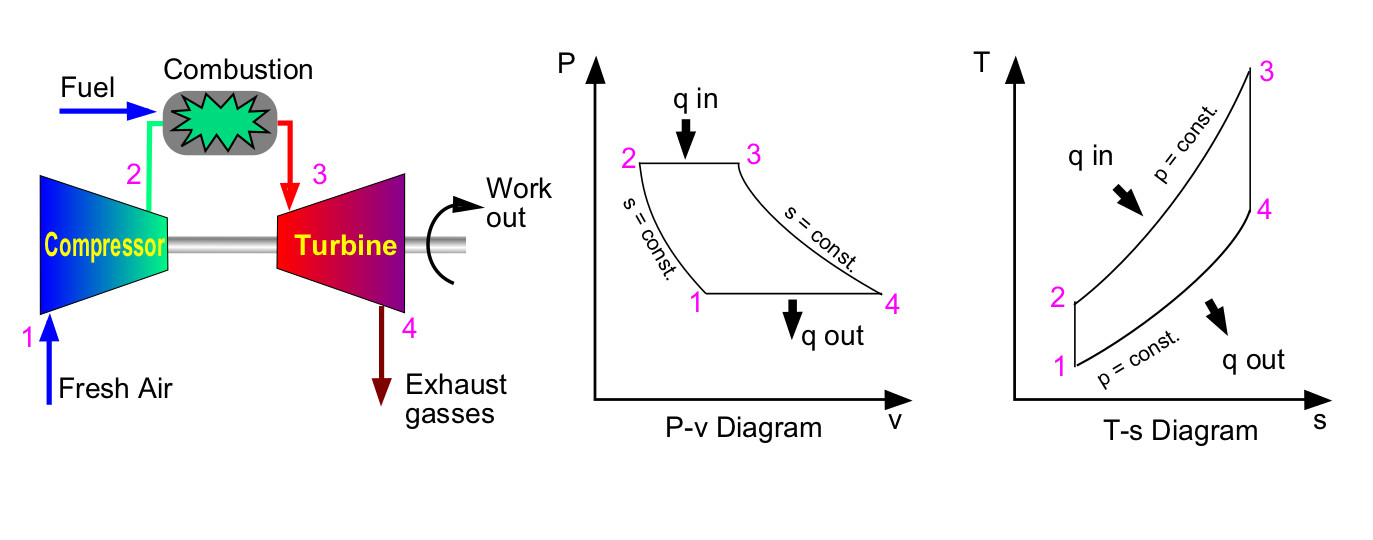
\includegraphics[width=\textwidth]{figures/review/brayton_cycle.jpg}
  \caption{Diagrams and plant layout of an idealized Brayton cycle\label{fig:brayton_cycle} }
\end{figure}


The efficiency of the cycle can be calculated as:

\begin{equation}
  \eta_{t}=1-\frac{1}{\beta^{k-1}}
\end{equation}

The regular Brayton thermodynamic cycle proved itself not to be suited for a bottoming cycle type of application. Of particular importance for waste heat recovery applications is the \emph{Super-critical CO\textsubscript{2}} (sCO2) Brayton cycle. Researchers claim \cite{Kimzey2012} that an sCO2 power cycle could potentially exhibit a higher thermal efficiency than steam cycles when operating between the same maximum and minimum cycle temperatures. In addition, the high energy density of sCO2 suggests that the size requirements for the turbomachinery used in an sCO2 power cycle could potentially be much lower than those used in steam cycle generation, which may result in lower capital costs. To date, most research in the field has been dedicated to the use of sCO2 as the primary power cycle in nuclear applications, but relatively little research has been aimed toward developing an sCO2 cycle that is well-suited to bottoming cycle applications.

\subsection{Selection of the bottoming cycle}

After having introduced the three most common thermodynamic cycles that can be employed as bottoming cycle, it's necessary to understand the up and downsides of the three in order to select the better one for the use case considered in this thesis.

The choice between the two different Rankine Cycles is basically reduces to the selection of the most appropriate working fluid. The choice of the working fluid to be used in the cycle depends on a number of factors, e.g thermodynamic efficiency, environmental protection, safety, process-related and economic issues.

The steam Rankine cycle is the most reliable and simple configuration considered, it has a high efficiency due to the very small work required for the pump. Water is widely available, cheap and does not present any issue in form of toxicity or environmental harm potential. The biggest downside of the selection of water is the huge latent heat of vaporization. According to Arias at al. \cite{Arias2006}, water is not suited to recover heat when used as a working fluid because of the mismatch between the low temperature of engine coolant and high boiling temperature of water. Water has been used in the fist generation of BMW's Rankine system \cite{Freymann2008}, the \emph{Turbosteamer}, to harvest energy from exhaust gases, while ethanol was used in a separate loop for engine coolant waste heat recovery. In the second generation Turbosteamer \cite{Freymann2012}, water is only been heated by the exhaust gases. This is because water works best when used for high exhaust gas temperature, from \SI{500}{\celsius} to \SI{800}{\celsius}. Water required also superheating to avoid turbine blade erosion, if turbine is selected as expander, but the high degree of superheating makes it less practical for the automotive application due to the variation of exhaust temperature at different load conditions. Besides, its high freezing point (\SI{0}{\celsius}) cannot meet the standard automotive working temperature range (\SI{-40}{\celsius} to \SI{85}{\celsius}).

Organic Rankine Cycle shows a much better potential for waste heat recovery in automotive applications. The low boiling point of the organic fluid allows to recover efficiently low-grade waste heat. The dry/isentropic refrigerants are widely used in small-scale RC applications because of their good heat transfer properties, excellent thermal stability and low viscosity. They are generally non-flammable, which is a big advantage for automotive application and compatible with most materials. Under typical low temperature ambient conditions they do not freeze, which is a major concern with water. Chammas and Clodic \cite{ElChammas2005} compared different organic fluids with water for RC application to hybrid vehicles, arguing that using water to recover automotive waste heat could lead to a complex system requiring large size equipment and high investment cost, which makes the study on organic working fluid necessary. Domingues et al. \cite{Domingues2012} compared R123 and R245fa with water as working fluid for vehicle RC waste heat recovery potential from exhaust gas. The study revealed the advantage of using water as working fluid to recover waste heat from exhaust gas of vehicles equipped with spark-ignition engine. However, it was also found that the heat exchanger effectiveness for R123 and R245fa is higher than that for water. Consequently, when the exhaust temperature is relatively low, organic fluids can be considered appropriate for vehicle RC application. Extensive work has also been poured in ORC + internal combustion engines combinations, leading to interesting fuel saving values.

The usage of organic fluids, such as refrigerants (i.e. R134a, R245fa, etc.) carries a few shortcomings. First, the intrisic property of dry/isentropic fluids reduce the area of net work in the T-s diagram, which means less power output compared to wet fluid, e.g. water. Second, to reduce the cooling load of the condenser, a recuperator is usually necessary to cool the superheated vapor to saturated state, increasing the system complexity and cost. Moreover, most organic fluids have relatively low thermal instability temperatures compared to water, therefore at high temperature and pressure the system might suffer chemical decomposition and deterioration. In addition, the current generation of refrigerants has a high global warming potential, which means that their use could be limited or banned in the near future.

The super-critical CO\textsubscript{2} Brayton cycle combines the advantages of both steam Rankine cycle and gas turbine system. In other words, the fluid is compressed in the incompressible region, and the higher turbine inlet temperature can be utilized with less material issues compared with the steam Rankine cycle. Therefore, the volumetric flow rate decreases as the fluid density is higher, resulting in 10 times smaller turbomachinery compared with the turbomachinery of a steam Rankine cycle \cite{Ahn2015}. In addition, researchers claim \cite{Kimzey2012} that an sCO2 cycle could potentially exhibit a higher thermal efficiency than steam cycle, when operating between the same maximum and minimum temperatures. A modeling research performed by Kimzey \cite{Kimzey2012} highlighted that the Brayton cycles are well suited to operating with a heat flux producing power source, but are not well suited to a sensible heat source, such as topping cycle exhaust. This is because this cycle is not truly effective at recovering waste heat: most Brayton cycles are not self-sustaining at operating temperatures below \SI{480}{\celsius}, a problem that revealed itself also in solar thermal plants. 

Given the above reasons, in this thesis an Organic Rankine Cycle has been selected as bottoming cycle to be modeled and coupled with the 3.6L V6 petrol engine Simulink model.

\section{Introduction to split cycle engines}

In the following chapter, an introduction to the basic concept of the split-cycle engine, and of alternative methodologies for recover waste heat will be provided. In the last decades engine improvements through friction reduction and improvements in the combustion system has been the main drivers, but savings will become increasingly difficult and costly \cite{Stanton2013}. The aim of this section is to introduce a different design that has the potential to achieve better results than the conventional one in terms of both efficiency and power density. The aforementioned approaches, combined with waste heat recovery, are likely to yield a maximum system efficiency of 45-50\%. Further improvements to efficiencies beyond 50\% require a fundamental change to ICE cycle \cite{Dong2015}.

\subsection{Basic principles}

In a conventional Otto cycle engine, each cylinder performs four strokes per cycle: intake, compression, power, and exhaust. This means that two revolutions of the crankshaft are required for each power stroke. The split-cycle engine divides these four strokes between two paired cylinders, a concept first described by Ricardo in 1908, and further developed by Carmelo Scuderi. Scuderi developed a modified version of the split-cycle engine, and filed the first patent for the \emph{Scuderi Split Cycle} (SSC) in 2001 \cite{Scuderi2003}, followed by supporting patents. The SSC concept divides the four strokes of a conventional combustion engine cycle over two paired cylinders. The first cylinder, referred to as the compressor, provides intake and compression strokes. The second cylinder, referred to as the expander, provides power and exhaust strokes. The two cylinders are connected by a crossover port through which the high pressure gas is transferred from the compressor cylinder to the expander cylinder between the compression and power strokes. The splitting of the compression and expansion strokes into separate cylinders has the potential to greatly improve the overall cycle efficiency. In Figure~\ref{fig:split_simple} \cite{gentili2014split}  is reported the general plan layout for a simple split cycle engine. In blue is the compression cylinder, in yellow the crossover, and in red the combustion cylinder.

\begin{figure}[ht]
  \centering
  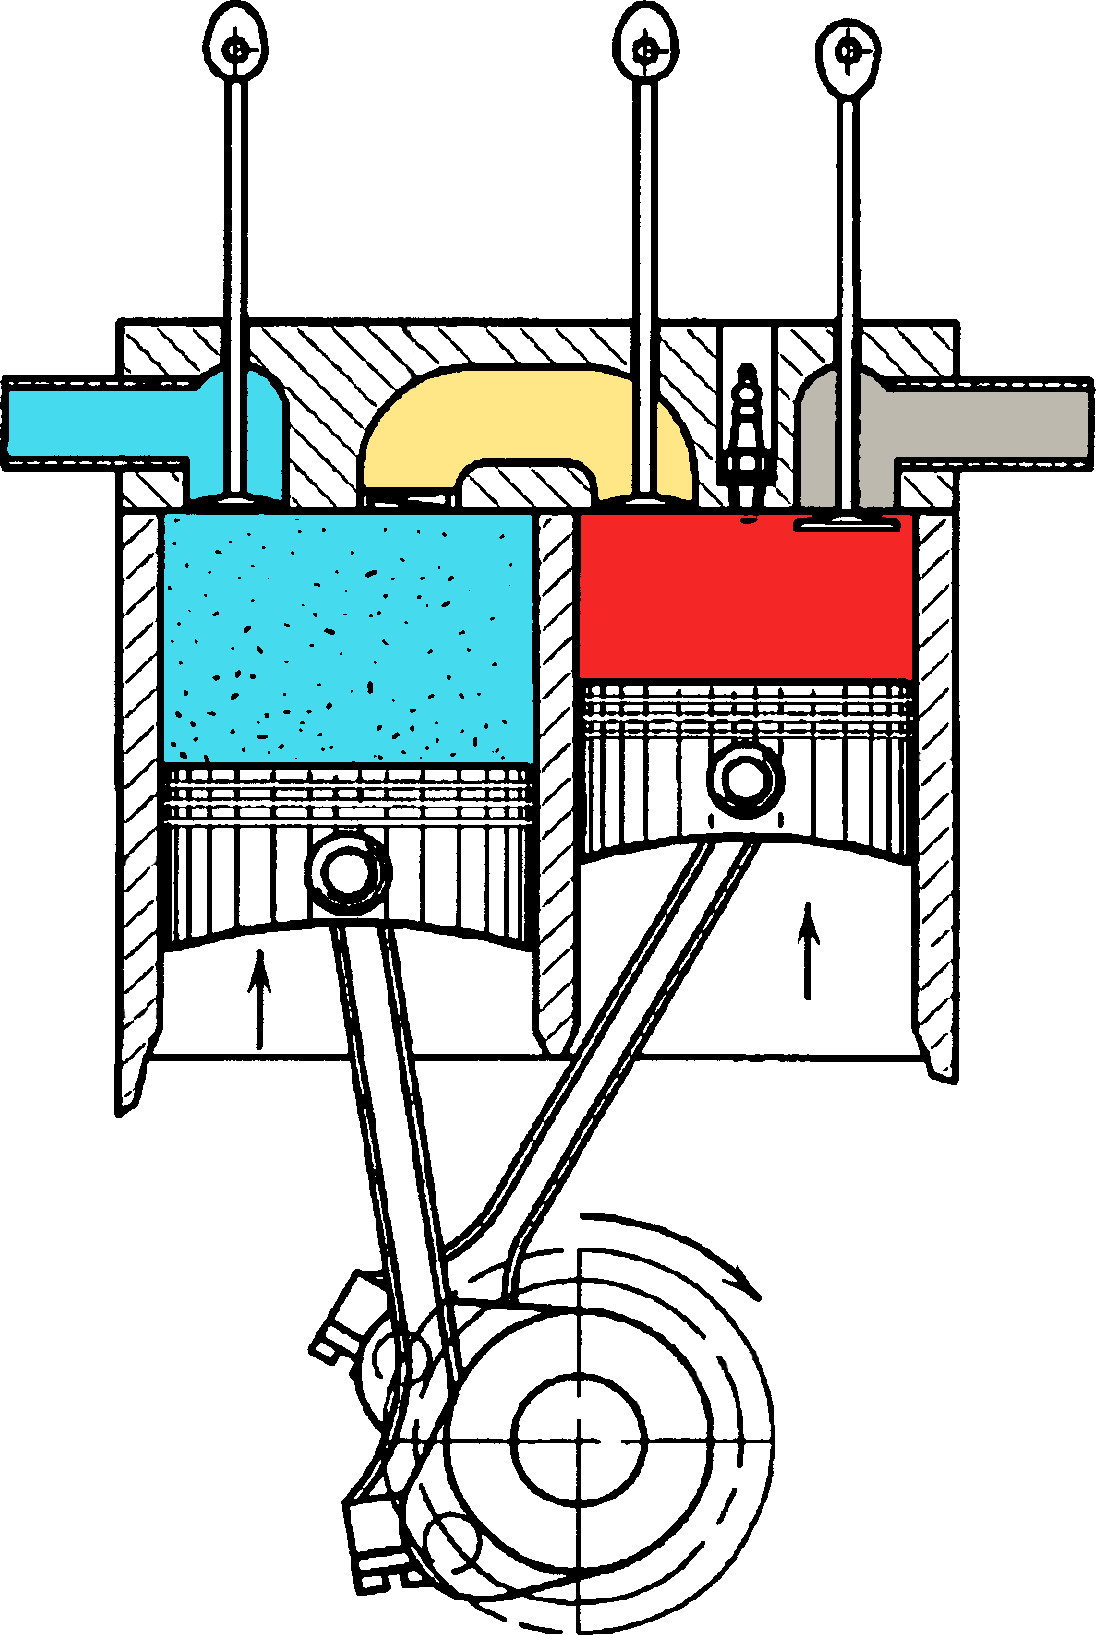
\includegraphics[width=0.5\textwidth]{figures/review/split_engine_view.png}
  \caption{Simplest plant layout for a split cycle engine\label{fig:split_simple} }
\end{figure}

A major functional benefit of the split-cycle as an internal combustion engine is the separation of compression and power strokes, which allows increased flexibility in optimizing these processes and designs. Other benefits are the ability for substantial Miller/Atkinson cycle type operation as extended expansion during the power stroke compared to compression stroke, or pressure charging the expander with the compressor, by use of differing compressor and expander displacements. Additionally, the crossover port arrangement enables charge motion, fuel and air mixing and combustion enhancement by means of the high pressure gas transfer from the crossover port to the expander. For SI applications, fuel injection can either be direct injection into the expander cylinder, or port injection into the crossover port during the gas transfer from the compressor into the expander (or both). Either method of injection results in less time for fuel chemical reactions leading to pre-ignition (or knock) than with intake port fuel injection used on conventional SI engines \cite{Phillips2011a}. The beneficial effects of such an engine configurations are also the reduction of the compression work, due to induction into a cool cylinder or direct cooling of the charge air during compression and the possibility of high pressure waste heat recovery between the compression and combustion cylinders.

Possible losses to be minimized in a split cycle engine are the flow pumping losses past the crossover valves and through the crossover ports, and energy losses due to heat transfer from the compressed air to the crossover port walls. Since the compressor cylinder has two cooler strokes, and the power cylinder has two hotter strokes, managing thermal loading is also a challenge for split cycle engines \cite{Phillips2011a}. 

Starting from the work of Coney et al. \cite{Coney2004}, the concept of isothermal compression has been applied to the split cycle engine to further improve its efficiency capabilities. Isothermal compression has the potential to reduce the after-compression temperature of the working fluid. By injecting the coolant media, such as liquid nitrogen or water, into the working fluid, the temperature of the compressed working fluid can be decreased significantly. It can be lower than the after-expansion temperature of the working fluid exiting the expansion cylinder. This allows to recover an increased amount of heat from the exhaust gases. This innovative methodology for waste heat recovery has been called \emph{intra-cycle waste heat recovery} (ICWHR) \cite{Coney2004, Dong2015, Morgan2016}. The split cycle engine structure design allows the compression and expansion processes to happen in separate chambers, and then heat recuperation is achieved through a recuperator installed between the two chambers. Due to the isothermal compression of the charge air, the temperature difference between the compression and expansion chamber is significant, allowing an efficient recuperation.

\subsection{Split-cycle engine operation}

In the following section the principles of engine operation for the split cycle will be explained, in terms of valve timing and crank angles. The timings are referred to the Scuderi version of the engine, and are based on the work of Phillips and al. \cite{Phillips2011a}.

\begin{figure}[ht]
  \centering
  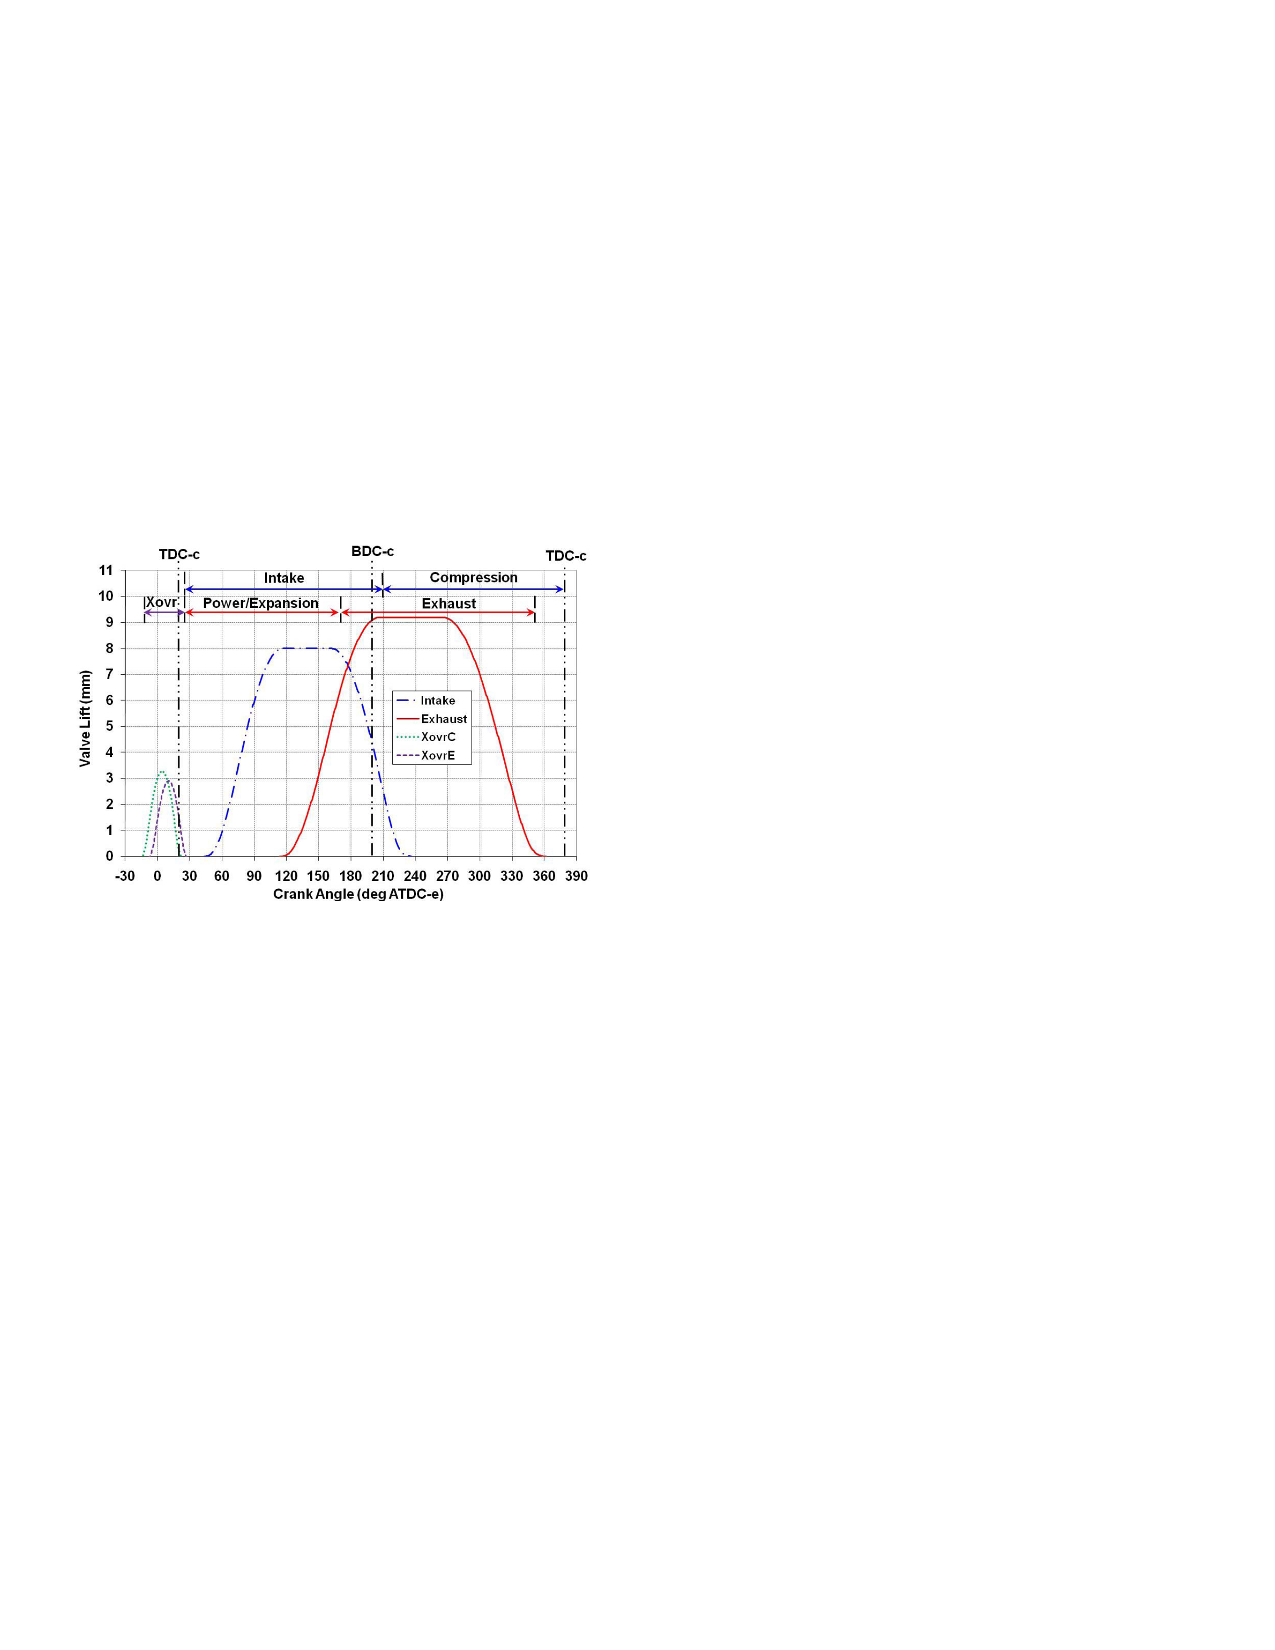
\includegraphics[width=\textwidth]{figures/introduction/split_timing.pdf}
  \caption{Valve events for SSC engine at 4000 RPM and full load conditions\label{fig:split_timing} }
\end{figure}

Figure~\ref{fig:split_timing} shows typical valve events for the engine. The compressor top dead center (TDC) is phased 20 degrees later than the expander TDC, and thus its crank angle scale is offset 20 degrees later than the expander scale shown. The Scuderi cycle begins at intake valve opening (IVO) of the compressor. For this operating point intake valve closing (IVC) is after BDC of both cylinders. Full variable valve actuation (VVA) is needed, so that the IVC varies with speed and load, and thus early IVC is used in combination with the intake throttle to control engine mass air flow. Compression takes place from IVC until TDC of the compressor cylinder, and overlaps the openings of the valves at the ends of the crossover (Xovr) ports, both at the compressor end (XovrC valves) as well as at the expander end (XovrE valves). In addition to the 4 phases of the conventional 4-stroke cycle, the SSC Xovr port provides a modulated high pressure gas transfer phase from compressor to expander cylinders between and overlapping the compression and power strokes. Prior to or slightly after XovrE valves open, fuel injection begins into the Xovr ports just ahead of the XovrE valves, and air and fuel mix enters the expander cylinder. As XovrE valves are nearly closed, spark ignition begins the power stroke. The power stroke ends when the exhaust valve opens (EVO) in the expander cylinder; the valve closes (EVC) just before TDC-e, ending the Scuderi cycle. Note that with fully variable intake and exhaust valve events, IVO, IVC, EVO and EVC timings can be varied with engine speed and load to optimize performance.

As the combustion takes place in an expanding cylinder, the peak temperatures are significantly lower than in a conventional engine leading to greatly reduced NOx formation. All gas-exchange and thermodynamic events are repeated every engine revolution such that the SSC can be viewed as a 4-stroke engine operating over two simultaneous 2-stroke cycles.
After

\subsection{Intra-cycle Waste Heat Recovery}

In this section the advantages and some implementation aspects of ICWHR will be presented and discussed. Figure~\ref{fig:ICWHR_vs_ORC}a shows the different energy fluxes that are related to an integrated waste heat recovery and to a bottoming cycle recovery.

\begin{figure}[ht]
  \centering
  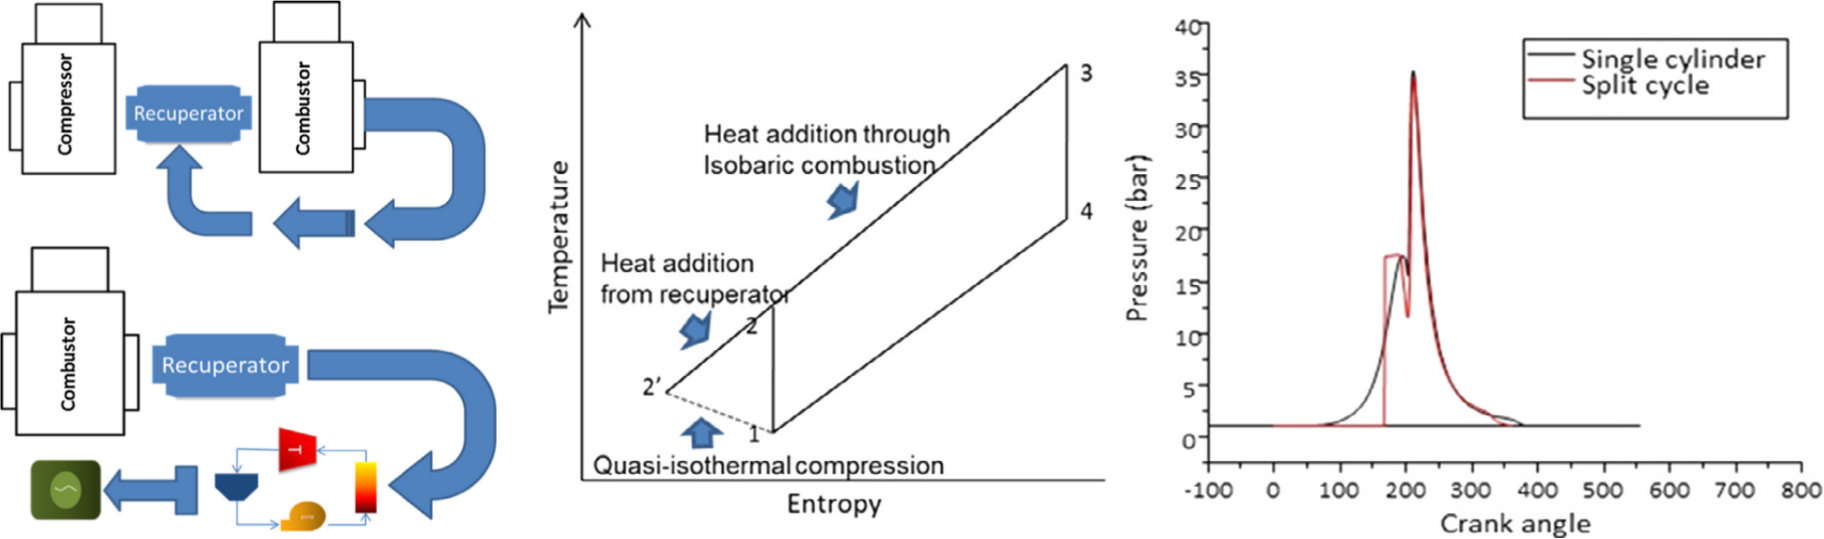
\includegraphics[width=\textwidth]{figures/review/ICWHR_vs_ORC.pdf}
  \caption{a) Comparison of the energy fluxes between an intra-cycle waste recovery and bottoming cycle type recovery, b) T-s and p-crank angle diagram for a split cycle engine with ICWHR\label{fig:ICWHR_vs_ORC} }
\end{figure}

As shown in Figure~\ref{fig:ICWHR_vs_ORC}b, the T-s diagram of the split cycle with the addition of the ICWHR is slightly different from the one showed before in Figure~\ref{fig:split_simple} due to the quasi-isothermal nature of the compression and the heat addiction coming from the recuperator.

A quasi-isothermal compression can be achieved by means of injection of water, or liquid nitrogen, during the compression phase in the first cylinder. Through the heat transfer between the intake air and the water spray droplets, the air temperature at the end of the compression stage can be decreased. The remaining liquid at the end of the compression phase can be removed using a separator.

\begin{figure}[ht]
  \centering
  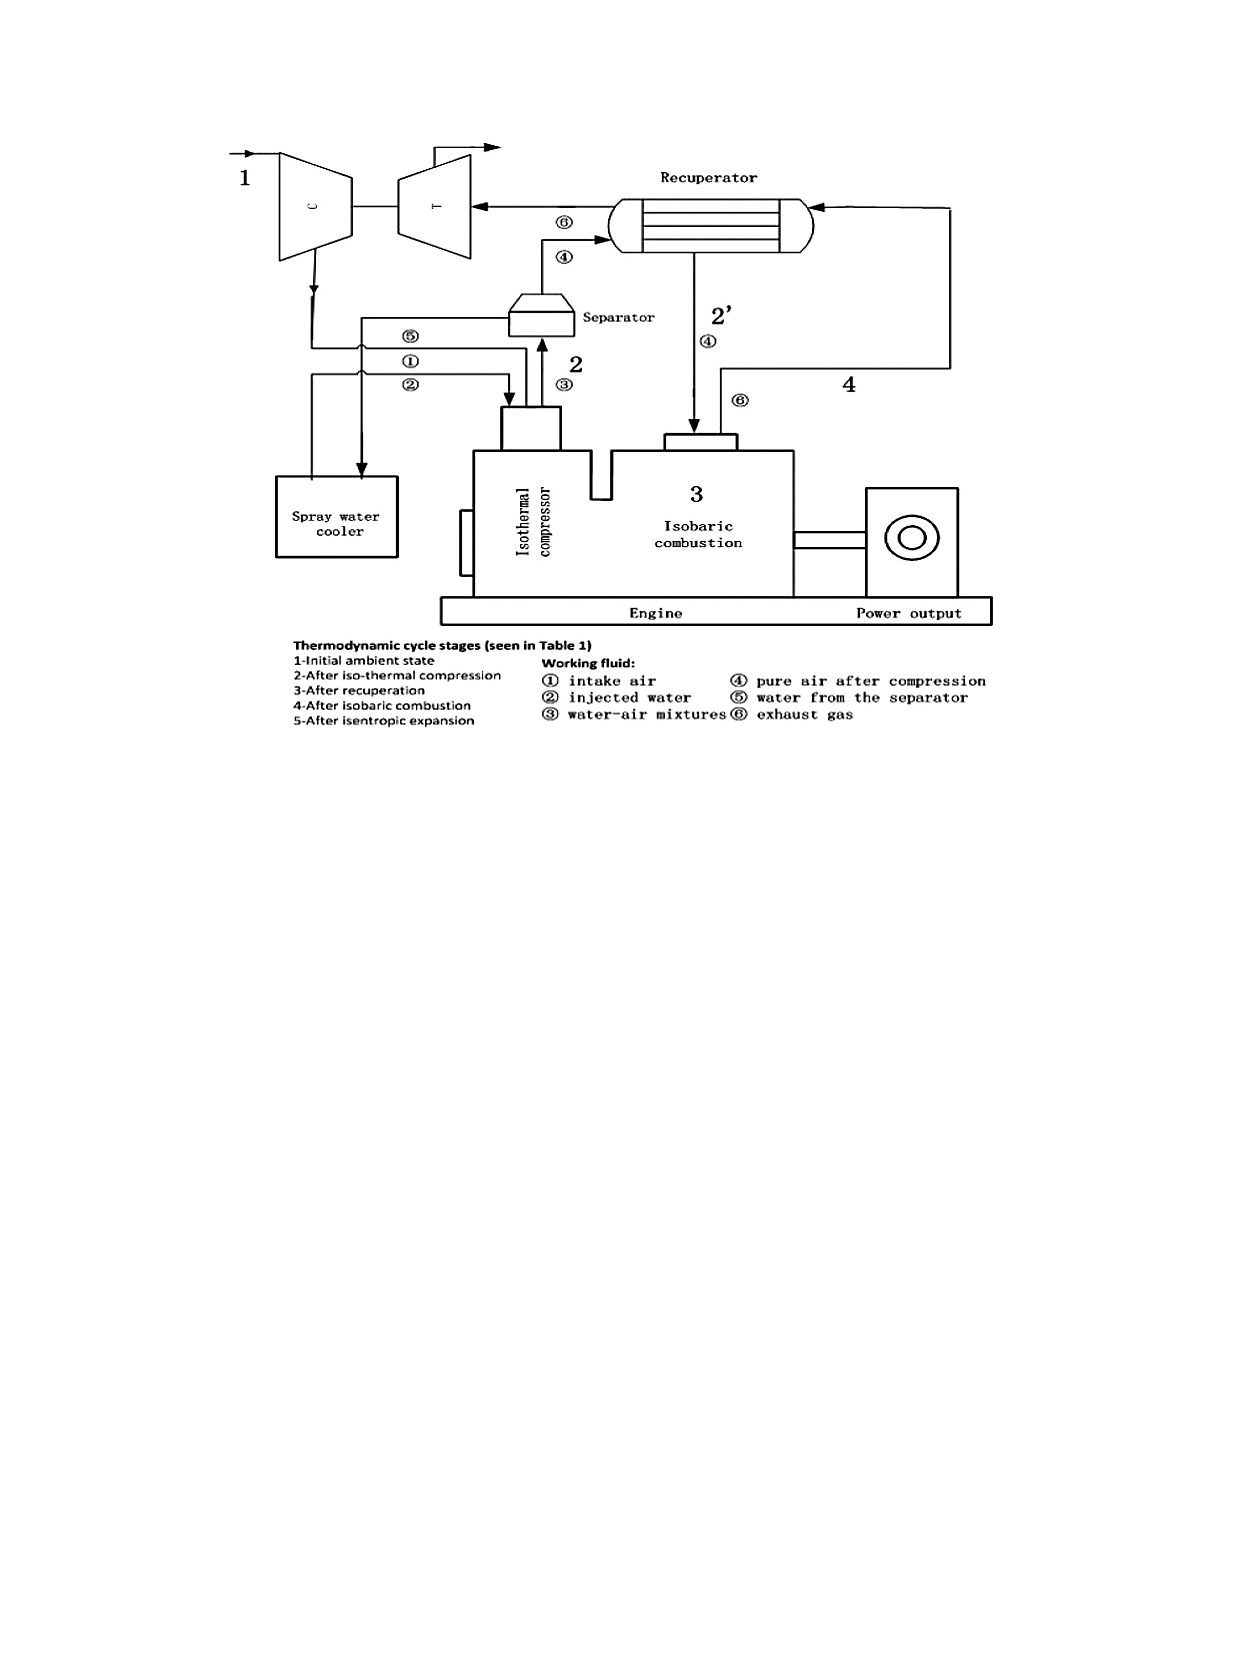
\includegraphics[width=0.8\textwidth]{figures/review/split_ICWHR_layout.pdf}
  \caption{Schematic of the engine equipped with quasi-isothermal compression and ICWHR\label{fig:split_ICWHR_layout} }
\end{figure}

In Figure~\ref{fig:split_ICWHR_layout} the layout of the engine with quasi isothermal-compression and ICWHR is shown. Ambient air (1) is pre-compressed in  turbocharger, and then sent to the reciprocating compression cylinder (2). Water is injected into the cylinder to cool down the air during compression, resulting in a quasi-isothermal compression process. After the compression stage (3), a high pressure two-phase water/air mixture leaves the isothermal compressor, and the water is recovered in a separator. The liquid water is cooled and sent back to a water tank (5). A recuperator is installed downstream the separator to heat the high-pressure air (4). Within the recuperator, the air is heated by the exhaust flow (7), and then an intra-cylinder heat recovery process is achieved. After the recuperation process (6), the fully preheated compressed air is fed to the combustion cylinders. As the combustion chamber intake valve opening time (IVO) is near to top dead centre (TDC), the diffusion of the combustion flame occurs in the expansion stroke of the cylinder. As a result, the combustion peak pressure is not increased significantly and a quasi-isobaric combustion process can be assumed. At the end of the expansion stage, the cylinder pressure is very close to the pressure in the exhaust pipe (7), so the exhaust stroke can be assumed as nearly isobaric as well. Based on the above processes, a complete split cycle is achieved \cite{Dong2015}.

%%% Local Variables:
%%% mode: latex
%%% TeX-engine: xetex
%%% TeX-master: "thesis"
%%% End:
